\subsection{Overview}
Planning for different kits is a major problem area in building a
flexible kitting workstation. Therefore, one area of focus for the
authors is metrics and test methods for planning for
kitting.  A test method is being developed that will be suitable for
comparing the performance of different kitting planning systems.  To build
such a test method, certain system prerequisites are necessary for the planning
system under test as well as for the hardware that will be utilized in
the implementation of the test method.
In order to provide for a consistent test metric, the  system system under
test needs a standardized representation for three sets of data:
\begin{itemize}
\item a representation for the initial conditions in the kitting workstation
 from which planning starts (the initial state)

\item a representation for the desired final conditions in the kitting
workstation after the plan has been executed (the goal state)

\item a representation for a plan to get from the initial state to the goal
state.
\end{itemize}

The first two representations are of the same nature: a description
primarily of objects and their locations. Hence, the same representation
may be used for both. Details follow shortly.

The representation of a plan is of a different nature. A plan is primarily
a description of actions that change one kitting workstation state to
another. Since the only active element in the model of a kitting
workstation is a one-armed robot, the plan model is a sequential
list of actions for a robot to perform.

\subsection{Kitting Workstation Data Representation}
Conceptually, the kitting workstation model is an object model as found in
several object oriented programming languages (C++, for example
\cite{Stroustrup.2000}).  That is:
\begin{itemize}
\item the model consists primarily of class definitions,
\item a class defines a type of thing,
\item classes have attributes (``elements'' in XML schema language),
\item the class definition gives the class (or data type) of each attribute,
\item some attributes may occur optionally or multiple times,
\item some classes are derived from others; thus, there is a derivation
 hierarchy,
\item a derived class has all the attributes of its parent plus, possibly,
  some of its own,
\item if class B is derived from class A, then if the type of an attribute
  is class A, an instance of class B may be used as the value of the attribute,
\item the model does not use multiple inheritance,
\item the model also uses primitive data types such as numbers and strings,
  and provides for defining specialized data types by putting constraints
  on primitive data types.
\end{itemize}

A complete hierarchical list of the classes used in the kitting workstation
model is shown in Figure~\ref{fig:ClassHierarchy}. In the list, there are two
top-level classes, SolidObject and DataThing. All other classes are
derived. Each class that is indented in the list is derived from the first
less indented class above it. For example, PartsBin is derived from
BoxyObject, and BoxyObject is derived from SolidObject. The figure does not
show any attributes.

\begin{figure}[th]
\centering
\vspace{-3 mm}
\fbox{
\begin{minipage}{3.2in}
\tt
\begin{tabbing}
xx\=xx\=xx\=\kill
SolidObject\\
\>BoxyObject\\
\>\>KitTray\\
\>\>LargeContainer\\
\>\>PartsBin\\
\>\>PartsTray\\
\>\>WorkTable\\
\>EndEffector\\
\>\>GripperEffector\\
\>\>VacuumEffector\\

\>\>\>VacuumEffectorMultiCup\\
\>\>\>VacuumEffectorSingleCup\\
\>EndEffectorHolder\\
\>Kit\\
\>KittingWorkstation\\
\>LargeBoxWithEmptyKitTrays\\
\>LargeBoxWithKits\\
\>Part\\
\>PartsTrayWithParts\\
\>Robot\\
DataThing\\
\>BoxVolume\\
\>KitDesign\\
\>PartRefAndPose\\
\>PhysicalLocation\\
\>\>PoseLocation\\
\>\>\>PoseLocationIn\\
\>\>\>PoseLocationOn\\
\>\>\>PoseOnlyLocation\\
\>\>RelativeLocation\\
\>\>\>RelativeLocationIn\\
\>\>\>RelativeLocationOn\\
\>Point\\
\>ShapeDesign\\
\>StockKeepingUnit\\
\>Vector\\
\end{tabbing}
\rm
\vspace{-3 mm}
\end{minipage}
}
\caption{Kitting Workstation Model Class Hierarchy}
\label{fig:ClassHierarchy}
\end{figure}

The structure of the kitting workstation class (or type) is shown in
Figure~\ref{fig:WorkstationModel}. The figure shows the names of the
attributes of a kitting workstation. The first three attributes (Name,
PrimaryLocation and SecondaryLocation) are inherited from the SolidObject
class. The rest of the attributes are specific to the kitting workstation
class. The AngleUnit, LengthUnit, and WeightUnit apply to all quantities in
a data file that are in terms of those unit types. No other unit types are
used in the model.

In Figure~\ref{fig:WorkstationModel} and similar figures (which were
generated by XMLSpy
\footnote{Certain commercial/open source software and tools are identified in this paper in order to explain our research. Such identification does not imply
recommendation or endorsement by the authors, nor does it imply that the software tools identified are necessarily the best available for the purpose.}
 from XML schemas), a dotted line around a box
means the attribute is optional (may occur zero times), while a \sf
..infinity \rm underneath a box means it may occur more than once, with no
upper limit on the number of occurrences.

\begin{figure}[t!]
\centering
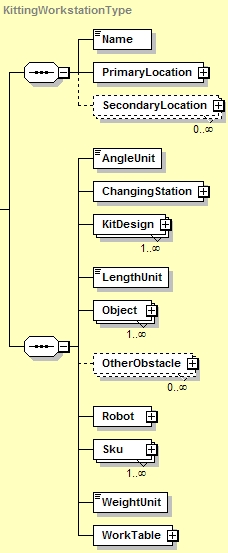
\includegraphics[width=3.166in]{images/kittingModelSmallCropped.jpg}
\caption{Kitting Workstation Model}
\label{fig:WorkstationModel}
\end{figure}

The types (i.e. classes or datatypes) of the attributes of a kitting
workstation are not shown on Figure~\ref{fig:WorkstationModel}. The
structures of several of the attributes are shown on the following figures:
\begin{itemize}
\item ChangingStation -- EndEffectorChangingStationType:
  Figure~\ref{fig:ChangingStation}
\item KitDesign -- KitDesignType: Figure~\ref{fig:KitDesign}
\item Object -- LargeBoxWithEmptyKitTraysType Figure~\ref{fig:LBWEKT},
  LargeBoxWithKitsType Figure~\ref{fig:LBWK}, and PartsTrayWithParts
  Figure~\ref{fig:PTWP}
\item Robot -- RobotType Figure~\ref{fig:Robot}
\item Sku -- StockKeepingUnitType Figure~\ref{fig:SKU}
\item WorkTable -- WorkTableType Figure~\ref{fig:WorkTable}.
\end{itemize}

The type of the Object elements of a kitting workstation is
SolidObject. That is an abstract class not intended to be
instantiated. Hence, the figures \ref{fig:ChangingStation} through
\ref{fig:WorkTable} show the structures of derived classes of
SolidObject that are intended to be used for instances of the Object
attribute.

\begin{figure}[htb!]
\centering
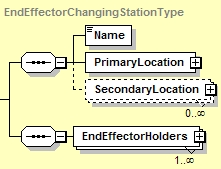
\includegraphics[width=3.166in]{images/changingStation.jpg}
\caption{Changing Station Model}
\label{fig:ChangingStation}
\end{figure}

\begin{figure}[htb!]
\centering
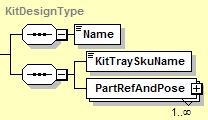
\includegraphics[width=3.1in]{images/kitDesign.jpg}
\caption{Kit Design Model}
\label{fig:KitDesign}
\end{figure}

\begin{figure}[htb!]
\centering
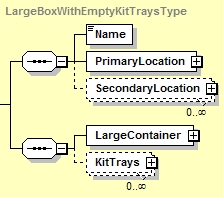
\includegraphics[width=3.1in]{images/largeBoxWithEmptyKitTrays.jpg}
\caption{Large Box With Empty Kit Trays Model}
\label{fig:LBWEKT}
\end{figure}

\begin{figure}[htb!]
\centering
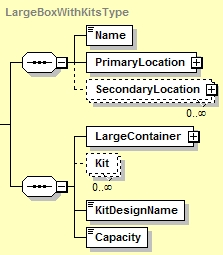
\includegraphics[width=3.1in]{images/largeBoxWithKits.jpg}
\caption{Large Box With Kits Model}
\label{fig:LBWK}
\end{figure}

\begin{figure}[htb!]
\centering
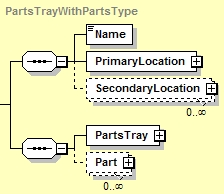
\includegraphics[width=3.1in]{images/partsTrayWithParts.jpg}
\caption{Parts Tray With Parts Model}
\label{fig:PTWP}
\end{figure}

\begin{figure}[htb!]
\centering
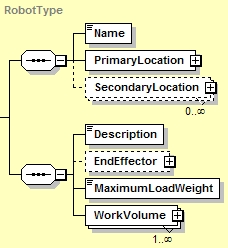
\includegraphics[width=3.166in]{images/robot.jpg}
\caption{Robot Model}
\label{fig:Robot}
\end{figure}

\begin{figure}[htb!]
\centering
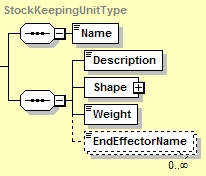
\includegraphics[width=3.166in]{images/sku.jpg}
\caption{Stock Keeping Unit Model}
\label{fig:SKU}
\end{figure}

\begin{figure}[htb!]
\centering
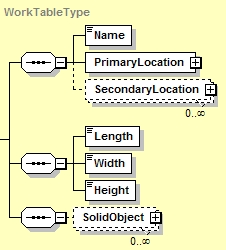
\includegraphics[width=3.166in]{images/worktable.jpg}
\caption{Work Table Model}
\label{fig:WorkTable}
\end{figure}

The robot model is simple and does not currently have any kinematics or
even any shape for the robot. It is likely that additional attributes will
be added in the future.

The kitting workstation model has been fully defined in each of two
languages: XML schema language \cite{Walmsley.2002},
\cite{XMLschemaPrimer}, \cite{XMLschemaStructures}, and Web Ontology
Language (OWL \it sic\rm) \cite{OWLoverview}, \cite{OWLprimer},
\cite{OWLspec}. Although the two models are conceptually identical, there
are some systematic differences between the models (in addition to
differences inherent in using two different languages).

\begin{itemize}
\item The complexType names (i.e. class names) in XML schema have the
  suffix ``Type'' added which is not used in OWL. This is so that the same
  names without the suffix can be used in XML schema language as element
  names without confusion.

\item All of the XML schema complexTypes have a ``Name'' element that is
  not present in OWL. It is not needed in OWL because names are assigned as
  a matter of course when instances of classes are created.

\item The movable objects that are in the kitting workstation are
  explicitly modeled in the XML schema model but not in the OWL model.

\item Attribute names in OWL have a prefix, as described below. The
  prefixes are not used in XML schema.
\end{itemize}
